\documentclass[12pt,a4paper]{article}
\usepackage[latin2]{inputenc}
\usepackage{graphicx}
\usepackage{ulem}
\usepackage{amsmath}
\usepackage{multicol}
\begin{document}
\begin{center}DAA432C \end{center}
\begin{center}Group-16 Assignment-01\end{center}

\begin{center}\textit{B. Tech IT 4$^{th}$ Semester Sec-B}
\end{center}

\begin{center}\textit{Indian Institute of Information Technology, 
Allahabad}\end{center}


\begin{multicols}{3}
\begin{center}IIT2019099\end{center}

\begin{center}Nitesh Rawat\end{center}

\begin{center}iit2019099@iiita.ac.in\end{center}

\begin{center}IIT2019100\end{center}

\begin{center}Maitry Jadiya\end{center}

\begin{center}iit2019100@iiita.ac.in\end{center}

\begin{center}IIT2019101\end{center}

\begin{center}Aryan Gupta\end{center}

\begin{center}iit2019101@iiita.ac.in\end{center}
\end{multicols}



\begin{multicols}{2}
\textbf{\textit{Abstract--- }In this report, we've shown the design and analysis of an algorithm that finds the missing element in an array that represents elements of an arithmetic progression using divide and conquer algorithm.}

\textbf{\textit{Keywords--- } Arithmetic progression, Divide and conquer, array, Binary Search }

\begin{center}I. INTRODUCTION\end{center}

This paper discusses about an algorithm that is  designed to  find the missing element in an array that represents elements of an arithmetic progression in order using divide and conquer approach.

\ \ \ \  An arithmetic sequence or progression(AP) is defined as a sequence of numbers in which for every pair of consecutive terms, the second number is obtained by adding a fixed number to the first one.

\ \ \ \ The array is already sorted either in increasing or decreasing order because, the elements of an array represent an arithmetic progression . 
 
\ \ \ \ This paper also contains the analysis about the time and space complexities of the algorithm. By the end of the paper, we will be able to understand all the components of algorithm design and will learn different ways of analysing the 
algorithms. 



\begin{center}II. ALGORITHM DESIGN-1\end{center}

\ \ \ \ The given problem can be solved by divide and conquer algorithm.Here we will be using the binary search approach .We will divide a given problem into smaller sub-problems and appropriately combine their solutions to get the solution to the main problem.  


\textit{  Approach:}Idea is to compare the elements of the given array(A) with an array whose elements are in proper arithmetic progression(B). We will find the first index of mismatch of A and B.The element of B in this index will give us our missing element.


\textit{  Algorithm:}

\newcounter{numberedCntA}
\begin{enumerate}
\item Find the mid element of the array every time search range is divided and initialise a result variable which will keep index of mismatched index.Input array A with a missing element and an array B which has elements in proper arithmetic progression(also having the missing element of A) is taken.
\item Check the values of array A and B on the mid index and if the elements are same then it would mean that no element was missing in the AP till this index.In this case start searching only to the right of mid(right half of the current search range).
\item Check the values of array A and B on the mid index and if the elements are unequal then store the index in result and keep checking to the left of mid(left half of the current search range) as the minimum index of mismatched value is required.If a smaller index of mismatch is found then result is updated with this index.
\item The value of result is returned after the range becomes zero.
\item After performing all the steps for all the subproblems, if the value of result variable is unchanged, then no element is missing in the array, otherwise, print the value of the result variable.
\setcounter{numberedCntA}{\theenumi}
\end{enumerate}

\begin{center}II. ALGORITHM DESIGN-2\end{center}

\ \ \ \ The given problem can be solved using divide and conquer approach which is similar to binary search.Basically we divide the given problem into smaller sub-problems and appropriately combine their solutions to get the solution to the main problem.  


\textit{  Approach:}The idea is to keep on checking the difference between the middle element and its adjacent elements unless the difference is not equal to the desired common difference.


\textit{  Algorithm:}

\newcounter{numberedCntB}
\begin{enumerate}
\item Find the mid element of the array and initialise an answer variable as the smallest integer that can be stored.
\item Check the difference between the middle element and its previous element. If the difference is not equal to the common difference of the AP, then store the missing number in an answer variable and make no further calls to the function, else proceed to next step.
\item Check the difference between the middle element and its next element. If the difference is not equal to the common difference of the AP, then store the missing number in a variable and make no further calls to the function, else proceed to next step.
\item If the current element is at its correct position, then divide the array into 2 halves, and perform the above steps in the later half, i.e. in the sub array from mid+1 till the end.
\item If the current element is not at its correct position, then divide the array into 2 halves, and perform the above steps in the first half, i.e. in the sub array from starting element till the mid.
\item After performing all the steps for all the subproblems, if the value of the answer variable is unchanged, then no element is missing in the array, otherwise, print the value of the answer variable.
\setcounter{numberedCntB}{\theenumi}
\end{enumerate}





\begin{center}III. PSEUDO CODE-1\end{center}


Function binarysearch(Argument a$[$$]$,Argument b$[$$]$, Argument n) 


\{ 
\quad initialize l =0 , h=n-1 ;
\quad  while l is less than h 
\{
\quad initialize m = l+((h-l) / 2);

\quad initialize res =-1;



\quad If a$[m]$==b$[m]$ l=m+1 range squeezes to right half


\quad Else if a$[m]$!=b$[m]$  res=mid, end=mid-1;


\}
 

\quad return res; 

end

\} 

\ \ Main function()\{ 

\quad Initialize integer array arr$[$$]$

\quad  Initialize n as size of array

\quad Input the elements of the array 

\quad d=a[n-1]-a[0]/n;
\quad b[0]=a[0] ; 
\quad for 1 to n b[i]=b[i-1]+d

\quad ans=binarysearch(a, b, n)

\quad print ans

\}



\} 


\begin{center}III. PSEUDO CODE-2\end{center}

\textit{ Declare global variable ans=INT\_MIN}

Function missingTerm(Argument a$[$$]$, Argument l, Argument h, Argument d) 


\{ 

\quad  If l is greater than or equal to h 

\quad\quad return ; 



\quad initialize m = (l + h) / 2

\quad initialize current=a$[0]$+m*d



\quad If a$[m]$-a$[m-1]$ is not equal to d and m is greater than 0

\quad\quad ans=a$[m-1]$+d 


\quad Else if a$[m+1]$-a$[m]$ is not equal to d and m+1 is less than h 

 \quad\quad ans=a$[m]$+d 
 
 \quad Else if a$[m]$ is equal to current
 
 \quad\quad missingTerm(a, m+1, h, d)
 
 \quad Else 
 
 \quad\quad missingTerm(a. l, m-1, d)

 

\quad return ; 

end

\} 

\ \ Main function()\{ 

\quad Initialize integer array arr$[$$]$

\quad  Initialize n as size of array

\quad Input the elements of the array 

\quad If n is less than 3, print "invalid input"

\quad Else \{

\quad Initialize d

\quad If a$[2]$-a$[1]$ is equal to a$[1]$-a$[0]$

\quad \quad d=a$[1]$-a$[0]$

\quad Else if a$[3]$-a$[2]$ is equal to a$[2]$-a$[1]$

\quad \quad d=a$[2]$-a$[1]$

\quad Else 

\quad \quad d=a$[1]$-a$[0]$

\quad missingTerm(a, 0, n, d)

\quad If ans is greater than INT\_MIN

\quad \quad print ans

\quad If ans is greater than INT\_MIN

\quad \quad print No term is missing

\}



\} 

\begin{center}IV. ALGORITHM ANALYSIS\end{center}


\ \ For both of the above approaches that are based on divide and conquer we are effectively dividing the array in the array into 2 halves and taking one of the two halves which is further divided into two halves, until the missing element is found.
 

\textit{ Calculating time complexity: }Assume that k (the function missing Term) is called k times. 

-  Assume the length of the array before any function calls is n. At each function call, the array is divided into 2 equal halves in approach-2 and in each iteration in the first approach its divided into two equal halves. 

- After the 1st function call, length of array becomes n/2. Also, in each next iteration in first method

- And according to the required condition one of the two halves is taken into consideration.

-  After the 2nd function call, the halved array from the previous step is divided again into two parts and length of array becomes n/4.

-  Similarly, After the 3rd function call, length of array becomes n/8.

-  Considering the same scenario after the k$^{th}$ function call, length of array becomes n/2$^{k}$.

-  Since the length of the array becomes 1 after k function calls(worst case) 

=$>$ n = 2$^{k}$

Hence k = log$_{2}$ (n)



Hence, the time complexity for both the above approaches is log$_{2}$
(n).

\textbf{Best Case-1 }

In this approach, the best case complexity is also O(log n) because the while loop will run always till the value of end becomes start.


\textbf{Best Case-2 }

When the element at the middle of the array is missing, i.e. the element at the middle position is not at the appropriate position in the AP, the best case arises. As we've found the required element in the 1$^{st}$ call so, there are no function calls involved and hence the time complexity would be O(1).

\textbf{Space Complexity-1 }

The space complexity of the algorithm will be O(n) because we're allocating the memory to a new array of the same size of the given array. So, extra space needed is O(n).

Space Complexity: O(n)

\textbf{Space Complexity-2 }

The space complexity of the algorithm will be O(log n) because the number of recursive calls to the function increase after the value of the length of array is halved.

Space Complexity: O(logn)





\end{multicols}
\begin{center}TABLE 1\end{center}

\begin{center}TIME COMPLEXITY OF  BINARY SEARCH APPROACHES \end{center}

\begin{table}[h]
\centering
\begin{tabular}{|l|l|l|}
\hline
\textbf{Class} & \textbf{Approch-1} & \textbf{Approch-2} \\
\hline
Worst case Complexity & O(log n) & O(log n) \\
\hline
Average case Complexity & O(log n) & O(log n) \\
\hline
Best Case Complexity & O(log n) & O(1) \\
\hline
\end{tabular}
\end{table}

\begin{center}TABLE 2\end{center}

\begin{center}SPACE COMPLEXITY OF  BINARY SEARCH APPROACHES\end{center}

\begin{table}[h]
\centering
\begin{tabular}{|l|l|l|}
\hline
\textbf{Class} & \textbf{Approch-1} & \textbf{Approch-2} \\
\hline
Space Complexity & O(n) & O(log n) \\
\hline
\end{tabular}
\end{table}

\begin{multicols}{2}


\begin{center}VI. PROFILING\end{center}



\textit{A. Time Complexity and Space Complexity:}

\ \ \ \ In this section, the  \textit{Posteriori Analysis or Profiling has been discussed. }
Now let us have the glimpse of time graph and then have a glimpse of the space graph.
\end{multicols}
\begin{figure}[h]
\centering
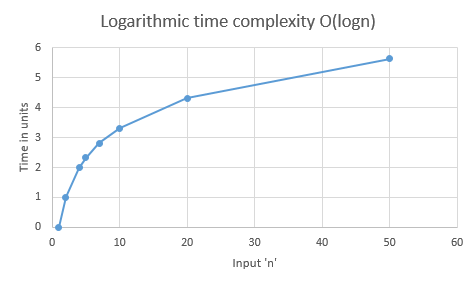
\includegraphics[width=8.44cm,height=6.64cm]{logarithmic-time-complexity.png}
\end{figure}

\begin{multicols}{2}
\begin{center}Figure 1: Time Complexity-1 and 2 \end{center}


\end{multicols}
\begin{figure}[h]
\centering
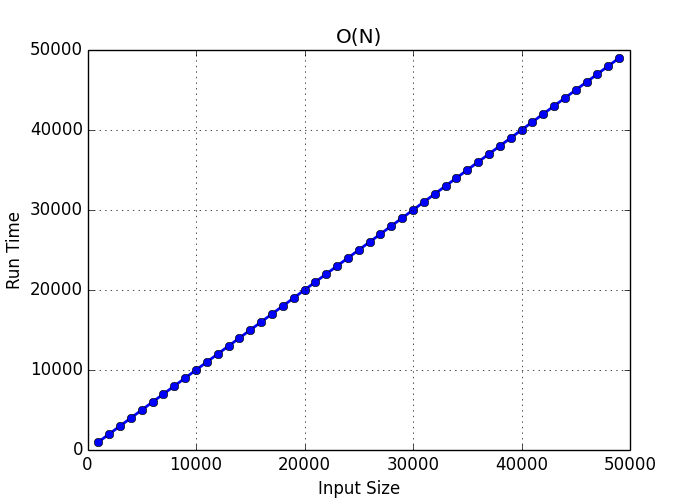
\includegraphics[width=8.44cm,height=6.73cm]{o-n.png}
\end{figure}

\begin{multicols}{2}
\begin{center}Figure 2: Space Complexity-1\end{center}


\end{multicols}
\begin{figure}[h]
\centering
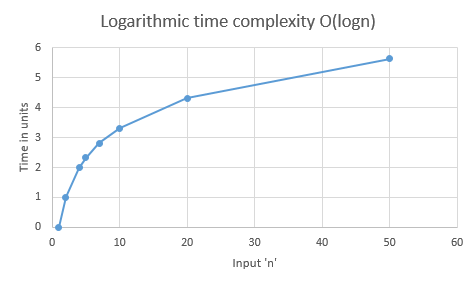
\includegraphics[width=8.44cm,height=6.73cm]{logarithmic-time-complexity.png}
\end{figure}

\begin{multicols}{2}
\begin{center}Figure 3: Space Complexity-2\end{center}



\begin{center}VII. CONCLUSION\end{center}

\ \ \ \ We can conclude that the second algorithm has the least time and space 
complexity to find the missing element in an array that represents elements of an arithmetic progression in order. 
The other one has same worst and average time complexity but best case time complexity of first approch is less than second one. Also,  it's space complexity is more than the other one.


\begin{center}REFERENCES\end{center}

$[$1$]$ Introduction to Algorithms / Thomas H. Cormen \ldots $[$et 
al.$]$. - 3$^{rd}$ edition.

$[$2$]$ The Design and Analysis of Algorithms (Pearson) by A V Aho, J E 
Hopcroft, and J D Ullman 

$[$3$]$ Algorithm Design (Pearson) by J Kleinberg, and E Tard

$[$4$]$ https://www.geeksforgeeks.org/find-missing-number-arithmetic-progression/

\end{multicols}







\end{document}
